% Options for packages loaded elsewhere
\PassOptionsToPackage{unicode}{hyperref}
\PassOptionsToPackage{hyphens}{url}
\PassOptionsToPackage{dvipsnames,svgnames,x11names}{xcolor}
%
\documentclass[
  letterpaper,
  DIV=11,
  numbers=noendperiod]{scrartcl}

\usepackage{amsmath,amssymb}
\usepackage{iftex}
\ifPDFTeX
  \usepackage[T1]{fontenc}
  \usepackage[utf8]{inputenc}
  \usepackage{textcomp} % provide euro and other symbols
\else % if luatex or xetex
  \usepackage{unicode-math}
  \defaultfontfeatures{Scale=MatchLowercase}
  \defaultfontfeatures[\rmfamily]{Ligatures=TeX,Scale=1}
\fi
\usepackage{lmodern}
\ifPDFTeX\else  
    % xetex/luatex font selection
\fi
% Use upquote if available, for straight quotes in verbatim environments
\IfFileExists{upquote.sty}{\usepackage{upquote}}{}
\IfFileExists{microtype.sty}{% use microtype if available
  \usepackage[]{microtype}
  \UseMicrotypeSet[protrusion]{basicmath} % disable protrusion for tt fonts
}{}
\makeatletter
\@ifundefined{KOMAClassName}{% if non-KOMA class
  \IfFileExists{parskip.sty}{%
    \usepackage{parskip}
  }{% else
    \setlength{\parindent}{0pt}
    \setlength{\parskip}{6pt plus 2pt minus 1pt}}
}{% if KOMA class
  \KOMAoptions{parskip=half}}
\makeatother
\usepackage{xcolor}
\setlength{\emergencystretch}{3em} % prevent overfull lines
\setcounter{secnumdepth}{-\maxdimen} % remove section numbering
% Make \paragraph and \subparagraph free-standing
\makeatletter
\ifx\paragraph\undefined\else
  \let\oldparagraph\paragraph
  \renewcommand{\paragraph}{
    \@ifstar
      \xxxParagraphStar
      \xxxParagraphNoStar
  }
  \newcommand{\xxxParagraphStar}[1]{\oldparagraph*{#1}\mbox{}}
  \newcommand{\xxxParagraphNoStar}[1]{\oldparagraph{#1}\mbox{}}
\fi
\ifx\subparagraph\undefined\else
  \let\oldsubparagraph\subparagraph
  \renewcommand{\subparagraph}{
    \@ifstar
      \xxxSubParagraphStar
      \xxxSubParagraphNoStar
  }
  \newcommand{\xxxSubParagraphStar}[1]{\oldsubparagraph*{#1}\mbox{}}
  \newcommand{\xxxSubParagraphNoStar}[1]{\oldsubparagraph{#1}\mbox{}}
\fi
\makeatother

\usepackage{color}
\usepackage{fancyvrb}
\newcommand{\VerbBar}{|}
\newcommand{\VERB}{\Verb[commandchars=\\\{\}]}
\DefineVerbatimEnvironment{Highlighting}{Verbatim}{commandchars=\\\{\}}
% Add ',fontsize=\small' for more characters per line
\usepackage{framed}
\definecolor{shadecolor}{RGB}{241,243,245}
\newenvironment{Shaded}{\begin{snugshade}}{\end{snugshade}}
\newcommand{\AlertTok}[1]{\textcolor[rgb]{0.68,0.00,0.00}{#1}}
\newcommand{\AnnotationTok}[1]{\textcolor[rgb]{0.37,0.37,0.37}{#1}}
\newcommand{\AttributeTok}[1]{\textcolor[rgb]{0.40,0.45,0.13}{#1}}
\newcommand{\BaseNTok}[1]{\textcolor[rgb]{0.68,0.00,0.00}{#1}}
\newcommand{\BuiltInTok}[1]{\textcolor[rgb]{0.00,0.23,0.31}{#1}}
\newcommand{\CharTok}[1]{\textcolor[rgb]{0.13,0.47,0.30}{#1}}
\newcommand{\CommentTok}[1]{\textcolor[rgb]{0.37,0.37,0.37}{#1}}
\newcommand{\CommentVarTok}[1]{\textcolor[rgb]{0.37,0.37,0.37}{\textit{#1}}}
\newcommand{\ConstantTok}[1]{\textcolor[rgb]{0.56,0.35,0.01}{#1}}
\newcommand{\ControlFlowTok}[1]{\textcolor[rgb]{0.00,0.23,0.31}{\textbf{#1}}}
\newcommand{\DataTypeTok}[1]{\textcolor[rgb]{0.68,0.00,0.00}{#1}}
\newcommand{\DecValTok}[1]{\textcolor[rgb]{0.68,0.00,0.00}{#1}}
\newcommand{\DocumentationTok}[1]{\textcolor[rgb]{0.37,0.37,0.37}{\textit{#1}}}
\newcommand{\ErrorTok}[1]{\textcolor[rgb]{0.68,0.00,0.00}{#1}}
\newcommand{\ExtensionTok}[1]{\textcolor[rgb]{0.00,0.23,0.31}{#1}}
\newcommand{\FloatTok}[1]{\textcolor[rgb]{0.68,0.00,0.00}{#1}}
\newcommand{\FunctionTok}[1]{\textcolor[rgb]{0.28,0.35,0.67}{#1}}
\newcommand{\ImportTok}[1]{\textcolor[rgb]{0.00,0.46,0.62}{#1}}
\newcommand{\InformationTok}[1]{\textcolor[rgb]{0.37,0.37,0.37}{#1}}
\newcommand{\KeywordTok}[1]{\textcolor[rgb]{0.00,0.23,0.31}{\textbf{#1}}}
\newcommand{\NormalTok}[1]{\textcolor[rgb]{0.00,0.23,0.31}{#1}}
\newcommand{\OperatorTok}[1]{\textcolor[rgb]{0.37,0.37,0.37}{#1}}
\newcommand{\OtherTok}[1]{\textcolor[rgb]{0.00,0.23,0.31}{#1}}
\newcommand{\PreprocessorTok}[1]{\textcolor[rgb]{0.68,0.00,0.00}{#1}}
\newcommand{\RegionMarkerTok}[1]{\textcolor[rgb]{0.00,0.23,0.31}{#1}}
\newcommand{\SpecialCharTok}[1]{\textcolor[rgb]{0.37,0.37,0.37}{#1}}
\newcommand{\SpecialStringTok}[1]{\textcolor[rgb]{0.13,0.47,0.30}{#1}}
\newcommand{\StringTok}[1]{\textcolor[rgb]{0.13,0.47,0.30}{#1}}
\newcommand{\VariableTok}[1]{\textcolor[rgb]{0.07,0.07,0.07}{#1}}
\newcommand{\VerbatimStringTok}[1]{\textcolor[rgb]{0.13,0.47,0.30}{#1}}
\newcommand{\WarningTok}[1]{\textcolor[rgb]{0.37,0.37,0.37}{\textit{#1}}}

\providecommand{\tightlist}{%
  \setlength{\itemsep}{0pt}\setlength{\parskip}{0pt}}\usepackage{longtable,booktabs,array}
\usepackage{calc} % for calculating minipage widths
% Correct order of tables after \paragraph or \subparagraph
\usepackage{etoolbox}
\makeatletter
\patchcmd\longtable{\par}{\if@noskipsec\mbox{}\fi\par}{}{}
\makeatother
% Allow footnotes in longtable head/foot
\IfFileExists{footnotehyper.sty}{\usepackage{footnotehyper}}{\usepackage{footnote}}
\makesavenoteenv{longtable}
\usepackage{graphicx}
\makeatletter
\newsavebox\pandoc@box
\newcommand*\pandocbounded[1]{% scales image to fit in text height/width
  \sbox\pandoc@box{#1}%
  \Gscale@div\@tempa{\textheight}{\dimexpr\ht\pandoc@box+\dp\pandoc@box\relax}%
  \Gscale@div\@tempb{\linewidth}{\wd\pandoc@box}%
  \ifdim\@tempb\p@<\@tempa\p@\let\@tempa\@tempb\fi% select the smaller of both
  \ifdim\@tempa\p@<\p@\scalebox{\@tempa}{\usebox\pandoc@box}%
  \else\usebox{\pandoc@box}%
  \fi%
}
% Set default figure placement to htbp
\def\fps@figure{htbp}
\makeatother

\KOMAoption{captions}{tableheading}
\makeatletter
\@ifpackageloaded{caption}{}{\usepackage{caption}}
\AtBeginDocument{%
\ifdefined\contentsname
  \renewcommand*\contentsname{Table of contents}
\else
  \newcommand\contentsname{Table of contents}
\fi
\ifdefined\listfigurename
  \renewcommand*\listfigurename{List of Figures}
\else
  \newcommand\listfigurename{List of Figures}
\fi
\ifdefined\listtablename
  \renewcommand*\listtablename{List of Tables}
\else
  \newcommand\listtablename{List of Tables}
\fi
\ifdefined\figurename
  \renewcommand*\figurename{Figure}
\else
  \newcommand\figurename{Figure}
\fi
\ifdefined\tablename
  \renewcommand*\tablename{Table}
\else
  \newcommand\tablename{Table}
\fi
}
\@ifpackageloaded{float}{}{\usepackage{float}}
\floatstyle{ruled}
\@ifundefined{c@chapter}{\newfloat{codelisting}{h}{lop}}{\newfloat{codelisting}{h}{lop}[chapter]}
\floatname{codelisting}{Listing}
\newcommand*\listoflistings{\listof{codelisting}{List of Listings}}
\makeatother
\makeatletter
\makeatother
\makeatletter
\@ifpackageloaded{caption}{}{\usepackage{caption}}
\@ifpackageloaded{subcaption}{}{\usepackage{subcaption}}
\makeatother

\usepackage{bookmark}

\IfFileExists{xurl.sty}{\usepackage{xurl}}{} % add URL line breaks if available
\urlstyle{same} % disable monospaced font for URLs
\hypersetup{
  pdftitle={CS546 Class Session 13 - Correlation network},
  pdfauthor={Trent VanHawkins},
  colorlinks=true,
  linkcolor={blue},
  filecolor={Maroon},
  citecolor={Blue},
  urlcolor={Blue},
  pdfcreator={LaTeX via pandoc}}


\title{CS546 Class Session 13 - Correlation network}
\author{Trent VanHawkins}
\date{2026-02-23}

\begin{document}
\maketitle


In this class session we are going to analyze gene expression data from
a human bladder cancer cohort, using python. We will load a data matrix
of expression measurements of 4,473 genes in 414 different bladder
cancer samples. These genes have been selected because they are
differentially expressed between normal bladder and bladder cancer (thus
more likely to have a function in bladder cancer specifically), but the
columns in the data matrix are restricted to bladder cancer samples (not
normal bladder) because we want to obtain a network representing
variation across cancers. The measurements in the matrix have already
been normalized to account for inter-sample heterogeneity and then log2
transformed. Our job is to compute Pearson correlation coefficients
between all pairs of genes, obtain Fisher-transformed \emph{z}-scores
for all pairs of genes, test each pair of genes for significance of the
\emph{z} score, adjust for multiple hypothesis testing, filter to
eliminate any pair for which \emph{R} \textless{} 0.75 or \emph{P}adj
\textgreater{} 0.01, load the graph into an \texttt{igraph.Graph}
object, and plot the degree distribution on log-log scale. We will then
answer two questions: (1) does the network look to be scale-free? and
(2) what is it's best-fit scaling exponent?

For this notebook, we will need \texttt{pandas}, \texttt{numpy},
\texttt{scipy.stats}, \texttt{matplotlib}, \texttt{pylab},
\texttt{statsmodels.sandbox.stats.multicomp}, \texttt{pycairo},
\texttt{igraph}, and \texttt{math}

\begin{Shaded}
\begin{Highlighting}[]
\ImportTok{import}\NormalTok{ pandas }\ImportTok{as}\NormalTok{ pd}
\ImportTok{import}\NormalTok{ numpy }\ImportTok{as}\NormalTok{ np}
\ImportTok{import}\NormalTok{ matplotlib.pyplot }\ImportTok{as}\NormalTok{ plt}
\ImportTok{import}\NormalTok{ scipy.stats, pylab, math}
\ImportTok{import}\NormalTok{ statsmodels.sandbox.stats.multicomp}
\ImportTok{import}\NormalTok{ cairo}
\ImportTok{import}\NormalTok{ igraph}
\end{Highlighting}
\end{Shaded}

Download the file
https://csx46.s3-us-west-2.amazonaws.com/bladder\_cancer\_genes\_tcga.txt
to the local file \texttt{bladder\_cancer\_genes\_tcga.txt}

\begin{Shaded}
\begin{Highlighting}[]
\OperatorTok{!}\NormalTok{curl https:}\OperatorTok{//}\NormalTok{csx46.s3}\OperatorTok{{-}}\NormalTok{us}\OperatorTok{{-}}\NormalTok{west}\OperatorTok{{-}}\FloatTok{2.}\ErrorTok{amazonaws}\NormalTok{.com}\OperatorTok{/}\NormalTok{bladder\_cancer\_genes\_tcga.txt }\OperatorTok{\textgreater{}}\NormalTok{ ..}\OperatorTok{/}\NormalTok{DataRaw}\OperatorTok{/}\NormalTok{bladder\_cancer\_genes\_tcga.txt}
\end{Highlighting}
\end{Shaded}

\begin{verbatim}
  % Total    % Received % Xferd  Average Speed   Time    Time     Time  Current
                                 Dload  Upload   Total   Spent    Left  Speed
100 29.9M  100 29.9M    0     0  21.0M      0  0:00:01  0:00:01 --:--:-- 21.0M
\end{verbatim}

Using \texttt{pandas.read\_csv}, load the tab-deliminted text file of
gene expression measurements (rows correspond to genes, columns
correspond to bladder tumor samples), into a data frame
\texttt{gene\_matrix\_for\_network\_df}.

\begin{Shaded}
\begin{Highlighting}[]
\NormalTok{gene\_matrix\_for\_network\_df }\OperatorTok{=}\NormalTok{ pd.read\_csv(}\StringTok{"../DataRaw/bladder\_cancer\_genes\_tcga.txt"}\NormalTok{, sep}\OperatorTok{=}\StringTok{"}\CharTok{\textbackslash{}t}\StringTok{"}\NormalTok{, index\_col}\OperatorTok{=}\DecValTok{0}\NormalTok{)}
\end{Highlighting}
\end{Shaded}

Use the \texttt{pandas.DataFrame.values} attribute to make a matrix
\texttt{gene\_matrix\_for\_network}. Print out the dimensions of the
matrix, by accessing its \texttt{shape} variable

\begin{Shaded}
\begin{Highlighting}[]
\NormalTok{gene\_matrix\_for\_network }\OperatorTok{=}\NormalTok{ np.array(gene\_matrix\_for\_network\_df.values)}
\NormalTok{gene\_matrix\_for\_network.shape}
\end{Highlighting}
\end{Shaded}

\begin{verbatim}
(4473, 414)
\end{verbatim}

Use \texttt{del} to delete the data frame, since we no longer need it
(save memory)

\begin{Shaded}
\begin{Highlighting}[]
\KeywordTok{del}\NormalTok{(gene\_matrix\_for\_network\_df)}
\end{Highlighting}
\end{Shaded}

Look at the online help for the \texttt{numpy.corrcoef} function, using
\texttt{help(np.corrcoef)}. When you pass a single argument \texttt{x}
which is a 2D ``array'' (i.e., a matrix), by default does
\texttt{corrcoef} compute coefficients for pairs of rows, or pairs of
columns?

Compute the 4,473 x 4,473 matrix of gene-gene Pearson correlation
coefficients, using \texttt{numpy.corrcoef} (this function treats each
row as a variable, so you don't have to do any transposing of the
matrix, unlike the situation in R).

\begin{Shaded}
\begin{Highlighting}[]
\NormalTok{gene\_matrix\_for\_network\_cor }\OperatorTok{=}\NormalTok{ np.corrcoef(gene\_matrix\_for\_network)}
\NormalTok{gene\_matrix\_for\_network\_cor.shape}
\end{Highlighting}
\end{Shaded}

\begin{verbatim}
(4473, 4473)
\end{verbatim}

Look at the online help for \texttt{numpy.fill\_diagonal}. Does it
return the modified matrix or modify the matrix argument in place?

Set the diagonal elements of the matrix to zero, using
\texttt{numpy.fill\_diagonal}

\begin{Shaded}
\begin{Highlighting}[]
\NormalTok{np.fill\_diagonal(gene\_matrix\_for\_network\_cor, }\DecValTok{0}\NormalTok{)}
\end{Highlighting}
\end{Shaded}

Look at the online help for \texttt{numpy.multiply}. Does it do
element-wise multiplication or matrix multiplication?

Look at the online help for \texttt{numpy.tri}. Does it modify a matrix
argument in-place or return a matrix? What is in the matrix that it
returns?

Set the upper-triangle of the matrix to zero, using
\texttt{numpy.multiply} and \texttt{numpy.tri} (for \texttt{numpy.tri},
you will want to use the single-asterisk argument syntax):

\begin{Shaded}
\begin{Highlighting}[]
\NormalTok{gene\_matrix\_for\_network\_cor }\OperatorTok{=}\NormalTok{ np.multiply(gene\_matrix\_for\_network\_cor,}
\NormalTok{                                          np.tri(}\OperatorTok{*}\NormalTok{gene\_matrix\_for\_network\_cor.shape))}
\end{Highlighting}
\end{Shaded}

Using \texttt{numpy.where}, get a tuple of two numpy.arrays containing
the row/col indices of the entries of the matrix for which \emph{R}
\textgreater= 0.75. Use array indexing to obtain the \emph{R} values for
these matrix entries, as a numpy array
\texttt{cor\_coeff\_values\_above\_thresh}.

\begin{Shaded}
\begin{Highlighting}[]
\NormalTok{inds\_correl\_above\_thresh }\OperatorTok{=}\NormalTok{ np.where(gene\_matrix\_for\_network\_cor }\OperatorTok{\textgreater{}} \FloatTok{0.75}\NormalTok{)}
\NormalTok{cor\_coeff\_values\_above\_thresh }\OperatorTok{=}\NormalTok{ gene\_matrix\_for\_network\_cor[inds\_correl\_above\_thresh]}
\end{Highlighting}
\end{Shaded}

Refer to Eq. (13.5) in the assigned readding for today's class (p9 of
the PDF). Obtain a numpy array of the correlation coefficients that
exceeded 0.75, and Fisher-transform the correlation coefficient values
to get a vector \texttt{z\_scores} of \emph{z} scores. Each of these
\emph{z} scores will correspond to an \textbf{edge} in the network,
unless the absolute \emph{z} score is too small such that we can't
exclude the null hypothesis that the corresponding two genes' expression
values are indepdenent (we will perform that check in the next step).

\begin{Shaded}
\begin{Highlighting}[]
\NormalTok{z\_scores }\OperatorTok{=}\NormalTok{ (}\DecValTok{1}\OperatorTok{/}\DecValTok{2}\NormalTok{)}\OperatorTok{*}\NormalTok{((}\DecValTok{1} \OperatorTok{+}\NormalTok{ cor\_coeff\_values\_above\_thresh)}\OperatorTok{/}\NormalTok{(}\DecValTok{1} \OperatorTok{{-}}\NormalTok{ cor\_coeff\_values\_above\_thresh))}
\end{Highlighting}
\end{Shaded}

Delete the correlation matrix object in order to save memory (we won't
need it from here on out).

\begin{Shaded}
\begin{Highlighting}[]
\KeywordTok{del}\NormalTok{(gene\_matrix\_for\_network\_cor)}
\end{Highlighting}
\end{Shaded}

Assume that under the null hypothesis that two genes are independent,
then sqrt(M-3)z for the pair of genes is an independent sample from the
normal distribution with zero mean and unit variance, where M is the
number of samples used to compute the Pearson correlation coefficient
(i.e., M = 414). For each entry in \texttt{z\_scores} compute a \emph{P}
value as the area under two tails of the normal distribution N(x), where
the two tails are x \textless{} -sqrt(M-3)z and x \textgreater{}
sqrt(M-3)z. (You'll know you are doing it right if z=0 means you get a P
value of 1). You will want to use the functions \texttt{numpy.abs} and
\texttt{scipy.stats.norm.cdf}, as well as the \texttt{math.sqrt}
function (in order to compute the square root).

\begin{Shaded}
\begin{Highlighting}[]
\BuiltInTok{len}\NormalTok{(z\_scores)}
\end{Highlighting}
\end{Shaded}

\begin{verbatim}
9916
\end{verbatim}

\begin{Shaded}
\begin{Highlighting}[]
\NormalTok{M }\OperatorTok{=} \DecValTok{414}
\NormalTok{P\_values }\OperatorTok{=} \DecValTok{2}\OperatorTok{*}\NormalTok{scipy.stats.norm.cdf(}\OperatorTok{{-}}\NormalTok{np.}\BuiltInTok{abs}\NormalTok{(z\_scores)}\OperatorTok{*}\NormalTok{math.sqrt(M}\OperatorTok{{-}}\DecValTok{3}\NormalTok{))}
\end{Highlighting}
\end{Shaded}

Adjust the P values for multiple hypothesis testing, using the
\texttt{statsmodels.sandbox.stats.multicomp.multipletests} function wth
\texttt{method="fdr\_bh"}

\begin{Shaded}
\begin{Highlighting}[]
\NormalTok{P\_values\_adj }\OperatorTok{=}\NormalTok{ statsmodels.sandbox.stats.multicomp.multipletests(P\_values, }
\NormalTok{                                                                 method}\OperatorTok{=}\StringTok{"fdr\_bh"}\NormalTok{)[}\DecValTok{1}\NormalTok{]}
\end{Highlighting}
\end{Shaded}

Verify that we don't need to drop any entries due to the adjusted P
value not being small enough (use \texttt{numpy.where} and
\texttt{len}); this should produce zero since we have M=414 samples per
gene.

\begin{Shaded}
\begin{Highlighting}[]
\BuiltInTok{len}\NormalTok{(np.where(P\_values\_adj }\OperatorTok{\textgreater{}=} \FloatTok{0.01}\NormalTok{)[}\DecValTok{0}\NormalTok{])}
\end{Highlighting}
\end{Shaded}

\begin{verbatim}
0
\end{verbatim}

Read the online help for the function \texttt{zip}. What does it do?

We want to pass our tuple of numpy arrays containing row and column
indices to \texttt{Graph.TupleList}; however, \texttt{Graph.TupleList}
accepts a tuple list, not a tuple of numpy arrays. So we need to make a
tuple list, using \texttt{zip}:

\begin{Shaded}
\begin{Highlighting}[]
\NormalTok{row\_col\_inds\_tuple\_list }\OperatorTok{=} \BuiltInTok{list}\NormalTok{(}\BuiltInTok{zip}\NormalTok{(inds\_correl\_above\_thresh[}\DecValTok{0}\NormalTok{],}
\NormalTok{                                   inds\_correl\_above\_thresh[}\DecValTok{1}\NormalTok{]))}

\CommentTok{\#\# [note this can be done more elegantly using the unary "*" operator:}
\CommentTok{\#\#    row\_col\_inds\_tuple\_list = list(zip(*inds\_correl\_above\_thresh))}
\CommentTok{\#\#  see how we only need to type the variable name once, if we use the unary "*" ]}
\end{Highlighting}
\end{Shaded}

Make an undirected graph from the row/column indices of the
(upper-triangle) gene pairs whose correlations were above our threshold,
using \texttt{igraph.Graph.TupleList}. Print a summary of the network,
as a sanity check, using the \texttt{igraph.Graph.summary} method.

Take a look at the first ten entries of
\texttt{row\_col\_inds\_tuple\_list}

\begin{Shaded}
\begin{Highlighting}[]
\NormalTok{row\_col\_inds\_tuple\_list[}\DecValTok{0}\NormalTok{:}\DecValTok{9}\NormalTok{]}
\end{Highlighting}
\end{Shaded}

\begin{verbatim}
[(np.int64(2), np.int64(0)),
 (np.int64(8), np.int64(1)),
 (np.int64(10), np.int64(9)),
 (np.int64(11), np.int64(0)),
 (np.int64(11), np.int64(2)),
 (np.int64(12), np.int64(0)),
 (np.int64(12), np.int64(2)),
 (np.int64(15), np.int64(2)),
 (np.int64(15), np.int64(12))]
\end{verbatim}

Make an \texttt{igraph.Graph} object called \texttt{final\_network}, by
passing \texttt{row\_col\_inds\_tuple\_list} to the class method
\texttt{igraph.Graph.TupleList}. As usual, print the graph summary using
\texttt{igraph.Graph.summary}.

\begin{Shaded}
\begin{Highlighting}[]
\NormalTok{final\_network }\OperatorTok{=}\NormalTok{ igraph.Graph.TupleList(row\_col\_inds\_tuple\_list, directed}\OperatorTok{=}\VariableTok{False}\NormalTok{)}
\NormalTok{final\_network.summary()}
\end{Highlighting}
\end{Shaded}

\begin{verbatim}
'IGRAPH UN-- 1394 9916 -- \n+ attr: name (v)'
\end{verbatim}

Plot the degree distribution on log-log scale; does it appear to be
scale-free?

\begin{Shaded}
\begin{Highlighting}[]
\NormalTok{degree\_dist }\OperatorTok{=}\NormalTok{ final\_network.degree\_distribution()}
\NormalTok{xs, ys }\OperatorTok{=} \BuiltInTok{zip}\NormalTok{(}\OperatorTok{*}\NormalTok{[(left, count) }\ControlFlowTok{for}\NormalTok{ left, \_, count }\KeywordTok{in}\NormalTok{ degree\_dist.bins()])}
\NormalTok{plt.scatter(xs, ys, marker}\OperatorTok{=}\StringTok{"o"}\NormalTok{)}
\NormalTok{ax }\OperatorTok{=}\NormalTok{ plt.gca()}
\NormalTok{ax.set\_yscale(}\StringTok{"log"}\NormalTok{)}
\NormalTok{ax.set\_xscale(}\StringTok{"log"}\NormalTok{)}
\NormalTok{plt.ylim((}\FloatTok{0.5}\NormalTok{,}\DecValTok{1000}\NormalTok{))}
\NormalTok{pylab.xlabel(}\StringTok{"k"}\NormalTok{)}
\NormalTok{pylab.ylabel(}\StringTok{"N(k)"}\NormalTok{)}
\NormalTok{pylab.show()}
\end{Highlighting}
\end{Shaded}

\pandocbounded{\includegraphics[keepaspectratio]{class13_correlnet_JTV_files/figure-pdf/cell-20-output-1.png}}

Use the \texttt{igraph.statistics.power\_law\_fit} function to estimate
the scaling exponent \emph{alpha} of the degree distribution:

\begin{Shaded}
\begin{Highlighting}[]
\NormalTok{igraph.statistics.power\_law\_fit(final\_network.degree()).alpha}
\end{Highlighting}
\end{Shaded}

\begin{verbatim}
1.5119389768928015
\end{verbatim}

Run the \texttt{community\_walktrap()} method on the
\texttt{final\_network} object to cluster the vertices, and assign the
resulting \texttt{igraph.clustering.VertexDendogram} object to variable
\texttt{comm\_res}.

\begin{Shaded}
\begin{Highlighting}[]
\NormalTok{comm\_res }\OperatorTok{=}\NormalTok{ final\_network.community\_walktrap()}
\end{Highlighting}
\end{Shaded}

\textbf{Plot} the dendrogram \texttt{comm\_res} using
\texttt{igraph.drawing.plot}

\begin{Shaded}
\begin{Highlighting}[]
\NormalTok{igraph.drawing.plot(comm\_res, bbox }\OperatorTok{=}\NormalTok{ (}\DecValTok{0}\NormalTok{,}\DecValTok{0}\NormalTok{,}\DecValTok{400}\NormalTok{,}\DecValTok{400}\NormalTok{))}
\end{Highlighting}
\end{Shaded}

\pandocbounded{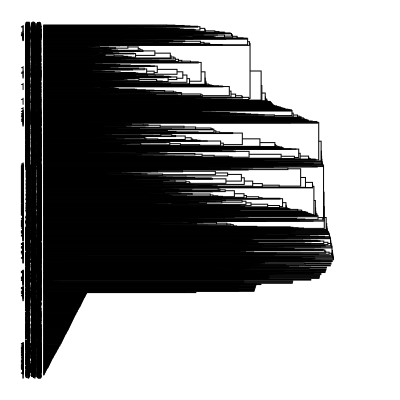
\includegraphics[keepaspectratio]{class13_correlnet_JTV_files/mediabag/class13_correlnet_JTV_files/figure-pdf/cell-23-output-1.pdf}}

Use \texttt{sorted} (with \texttt{reverse=True}) and the
\texttt{as\_clustering()} and \texttt{sizes()} methods (chained) to
examine sizes of the 20 largest clusters.

\begin{Shaded}
\begin{Highlighting}[]
\BuiltInTok{sorted}\NormalTok{(comm\_res.as\_clustering().sizes(), reverse}\OperatorTok{=}\VariableTok{True}\NormalTok{)[}\DecValTok{0}\NormalTok{:}\DecValTok{20}\NormalTok{]}
\end{Highlighting}
\end{Shaded}

\begin{verbatim}
[392, 209, 147, 29, 9, 9, 8, 7, 7, 7, 6, 6, 6, 5, 5, 5, 5, 5, 5, 5]
\end{verbatim}




\end{document}
